\documentclass[11pt,a4paper,danish]{article}
\usepackage[utf8]{inputenc} % Skal passe til editorens indstillinger
\usepackage[danish]{babel} % danske overskrifter
\usepackage[T1]{fontenc} % fonte (output)
\usepackage{lmodern} % vektor fonte
\usepackage{graphicx} % indsættelse af billeder
\usepackage{mathtools} % matematik - understøtter muligheden for at bruge \eqref{}
\usepackage[plainpages=false,pdfpagelabels,pageanchor=false]{hyperref} % aktive links
\usepackage{algpseudocode}
\usepackage{algorithm}
% \usepackage{pstool}
\hypersetup{
  pdfauthor={Peter Bay Bastian (s113119)},
  pdftitle={Hjemmeopgave 3},
  pdfsubject={01017 Diskret matematik}}
\usepackage{epstopdf}
\usepackage{memhfixc}% rettelser til hyperref
\usepackage{colortbl}
\usepackage{color}
\usepackage{listings}
\usepackage{textcomp}
\usepackage{amsfonts} 
\usepackage[usenames,dvipsnames]{pstricks}
\usepackage{pst-grad} % For gradients
\usepackage{pst-plot} % For axes
\usepackage{float}
\usepackage{fancyhdr}
\usepackage{ae}
\usepackage{amssymb}
\usepackage{tikz}

\newcommand{\closed}{child[white, level distance=5mm] {node[black] {$\times$}}}
\newcommand{\open}{child[white, level distance=5mm] {node[black] {$\bigcirc$}}}
\newcommand{\F}{\mathtt{F}}
\newcommand{\T}{\mathtt{T}}

\pagestyle{fancy}
\renewcommand{\headheight}{25.27927pt}
\renewcommand{\headrulewidth}{0.4pt}
\renewcommand{\footrulewidth}{0pt}
\fancyhead{}
\fancyhead[L]{\today\\Peter Bay Bastian (s113119)}
\fancyhead[R]{Hjemmeopgave 3\\02101 Diskret matematik E12}
\fancyfoot[C]{\thepage}

\title{Hjemmeopgave 3}
\author{Peter Bay Bastian (s113116)}

\begin{document}
	%\maketitle
	\noindent
	Opgaven er lavet i samarbejde med Kim Bo Rasmussen (s070808) og Mikkel Møller Nielsen Davidsen (s113116).

	%!TEX root = document.tex
\section*{Opgave A}
\begin{enumerate}
  \item
  Jeg benytter følgende propositionsvariable:
  \begin{itemize}
    \item $P_r$: P er ridder
    \item $Q_r$: Q er ridder
  \end{itemize}
  Hvis P ikke er en ridder må P være en bonde, da der kun findes to typer af mennesker på øen. Altså kan jeg udtrykke at P er en bonde ved $\lnot P_r$. Ligeledes kan jeg udtrykke at Q er en bonde ved $\lnot Q_r$.

  For at bestemme hvad P og Q er, ser jeg først på Ps svar på spørgsmålet. Man må kunne udtrykke at mindst én af dem er en bonde ved:
  \begin{equation}
    \label{A1:udsagn}
    \lnot P_r \lor \lnot Q_r
  \end{equation}
  Hvis \eqref{A1:udsagn} er sandt må $P_r$ være sandt, da P i så fald har talt sandt og derved ikke kan være en bonde. Hvis \eqref{A1:udsagn} er falsk må $P_r$ være falsk, da P i så fald har løjet og derved ikke kan være en ridder.

  Ligeledes må \eqref{A1:udsagn} være falsk hvis $P_r$ er falsk, og sandt hvis $P_r$ er sand.

  Altså må der være tale om en biimplikation, og situationen kan beskrives ved:
  \begin{equation}
    \label{A1:situation}
    P_r \leftrightarrow \lnot P_r \lor \lnot Q_r
  \end{equation}

  Jeg kan undersøge hvilke værdier der vil gøre \eqref{A1:situation} sand vha. tableau-metoden:
  \begin{equation*}
    \begin{tikzpicture}[level distance=8mm,sibling distance=50mm]
      \node {$P_r \leftrightarrow \lnot P_r \lor \lnot Q_r : \T\ \checkmark$}
      child {
        node {$P_r : \T$}
        child {
          node {$\lnot P_r \lor \lnot Q_r : \T\ \checkmark$}
          child {
            node {$\lnot P_r : \T\ \checkmark$}
            child {
              node {$P_r : \F$}
              \closed
            }
          }
          child {
            node {$\lnot Q_r : \T\ \checkmark$}
            child {
              node {$Q_r : \F$}
              \open
            }
          }
        }
      }
      child {
        node {$P_r : \F$}
        child {
          node {$\lnot P_r \lor \lnot Q_r : \F\ \checkmark$}
          child {
            node {$\lnot P_r : \F\ \checkmark$}
            child {
              node {$\lnot Q_r : \F$}
              child {
                node {$P_r : \T$}
                \closed
              }
            }
          }
        }
      };
    \end{tikzpicture}
  \end{equation*}

  Det ses at der kun en én åben, mættet gren, hvor $P_r$ er sand og $Q_r$ er falsk.

  Altså er P en ridder og Q en bonde.

  \item
  Jeg benytter følgende propositionsvariable:
  \begin{itemize}
    \item $A_r$: A er ridder
    \item $B_r$: B er ridder
  \end{itemize}

  Svaret A giver kan udtrykkes ved:
  \begin{equation}
    \lnot B_r \rightarrow \lnot A_r
  \end{equation}

  Ligesom før kan situationen beskrives ved en biimplikation mellem A og svaret A gav:
  \begin{equation}
    \label{A2:situation}
    B_r \leftrightarrow \left( \lnot B_r \rightarrow \lnot A_r \right)
  \end{equation}

  Undersøger hvilke værdier der opfylder \eqref{A2:situation} vha. tableau-metoden:
  \begin{equation*}
    \begin{tikzpicture}[level distance=8mm,sibling distance=50mm]
      \node {$A_r \leftrightarrow \left( \lnot B_r \rightarrow \lnot A_r \right) : \T\ \checkmark$}
      child {
        node {$A_r : \T$}
        child {
          node {$\lnot B_r \rightarrow \lnot A_r : \T\ \checkmark$}
          child {
            node {$\lnot B_r : \F\ \checkmark$}
            child {
              node {$B_r : \T$}
              \open
            }
          }
          child {
            node {$\lnot A_r : \T$}
            child {
              node {$A_r : \F$}
              \closed
            }
          }
        }
      }
      child {
        node {$A_r : \F$}
        child {
          node {$\lnot B_r \rightarrow \lnot A_r : \F\ \checkmark$}
          child {
            node {$\lnot B_r : \T$}
            child {
              node {$\lnot A_r : \F\ \checkmark$}
              child {
                node {$A_r : \T$}
                \closed
              }
            }
          }
        }
      };
    \end{tikzpicture}
  \end{equation*}

  Det ses at der kun er én åben, mættet gren, hvor $A_r$ er sand og $B_r$ er sand.

  Altså er både A og B riddere.

  \item
  Jeg benytter følgende propositionsvariable:
  \begin{itemize}
    \item $C_r$: C er ridder
    \item $C_k$: C er kannibal
    \item $D_r$: D er ridder
    \item $D_k$: D er kannibal
    \item $E_r$: E er ridder
    \item $E_k$: E er kannibal
  \end{itemize}

  Der er nu tre udsagn. Hele situationen kan opdeles i tre undersituationer, hvor hvert udsagn afhænger af om den der sagde det er en ridder. (Biimplikation ligesom før.)

  Jeg ser først på undersituationen for C. Givet at D oversætter korrekt, siger C at kun én af dem er en ridder. Det kan udtrykkes ved følgende, som jeg vælger at kalde $R_1$ pga. det lange udtryk:
  \begin{equation}
    \label{A3:Csvar}
    \begin{split}
      R_1 \equiv & \left( C_r \land \left( \lnot D_r \land \lnot E_r \right) \right) \lor\\
                 & \left( \lnot C_r \land \left( D_r \land \lnot E_r \right) \right) \lor\\
                 & \left( \lnot C_r \land \left( \lnot D_r \land E_r \right) \right)
    \end{split}
  \end{equation}

  E siger at D er en bonde og at E ikke er en kannibal. Det kan udtrykkes ved:
  \begin{equation}
    \label{A3:Esvar}
    \lnot D_r \land \lnot E_k
  \end{equation}

  D siger at D ikke er en kannibal, hvilket kan udtrykkes ved:
  \begin{equation}
    \label{A3:Dsvar}
    \lnot D_k
  \end{equation}

  Ligesom før kan situationen beskrives vha. biimplikationer. \eqref{A3:Csvar} afhænger først og fremmest af om C er en ridder (og derved taler sandt). Situationen for C kan da udtrykkes ved:
  \begin{equation}
    \label{A3:Csituation}
    \begin{split}
      C_r \leftrightarrow & \left( C_r \land \left( \lnot D_r \land \lnot E_r \right) \right) \lor\\
      & \left( \lnot C_r \land \left( D_r \land \lnot E_r \right) \right) \lor \left( \lnot C_r \land \left( \lnot D_r \land E_r \right) \right)
    \end{split}
  \end{equation}

  Da D stod for oversættelsen fra det C sagde, må \eqref{A3:Csituation} afhænge af hvorvidt D er en ridder. Det D selv sagde afhænger selvfølgelig også af om D er en ridder. Altså er C's situation en del af D's situation, og derved kan \eqref{A3:Csituation} og \eqref{A3:Dsvar} samles i et udtryk for D's situation:
  \begin{equation}
    \begin{split}
      D_r \leftrightarrow \lnot D_k \land ( C_r \leftrightarrow R_1 )
    \end{split}
  \end{equation}

  E's situation kan udtrykkes ved:
  \begin{equation}
    E_r \leftrightarrow \lnot D_r \land \lnot E_k
  \end{equation}

  Ved at samle situationerne for D, som indeholder situationen for C, og E kan jeg få et udtryk for den samlede situation ved:
  \begin{equation}
    \begin{split}
      \left( E_r \leftrightarrow & \lnot D_r \land \lnot E_k\right) \land \left( D_r \leftrightarrow \lnot D_k \land \left( C_r \leftrightarrow R_1 \right) \right)
    \end{split}
  \end{equation}

  Tableau-metoden:
  \begin{equation*}
    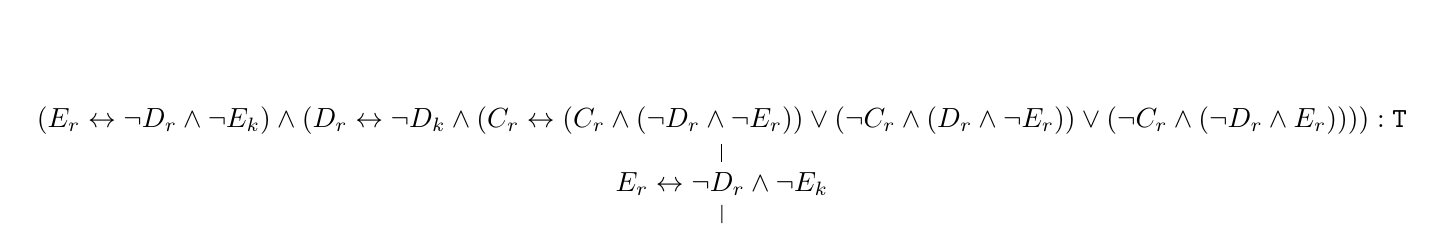
\begin{tikzpicture}[level distance=8mm,sibling distance=50mm]
      \node {$\left( E_r \leftrightarrow \lnot D_r \land \lnot E_k\right) \land (
      D_r \leftrightarrow \lnot D_k \land ( C_r \leftrightarrow \left( C_r \land \left( \lnot D_r \land \lnot E_r \right) \right) \lor
      \left( \lnot C_r \land \left( D_r \land \lnot E_r \right) \right) \lor \left( \lnot C_r \land \left( \lnot D_r \land E_r \right) \right) )) : \T$}
      child {
        node {$E_r \leftrightarrow \lnot D_r \land \lnot E_k$}
        child {
          node {$D_r \leftrightarrow \lnot D_k \land ( C_r \leftrightarrow \left( C_r \land \left( \lnot D_r \land \lnot E_r \right) \right) \lor
                \left( \lnot C_r \land \left( D_r \land \lnot E_r \right) \right) \lor \left( \lnot C_r \land \left( \lnot D_r \land E_r \right) \right) )$}
        }
      };
    \end{tikzpicture}
  \end{equation*}
\end{enumerate}
	%!TEX root = document.tex
\section*{Opgave B}
	%!TEX root = document.tex
\section*{Opgave C}
Jeg vil bevise følgende lemma gælder:
\begin{description}
  \item[Lemma 1] Formlerne A og B er logisk ækvivalente hvis og kun hvis formlen $A \leftrightarrow B$ er gyldig.
\end{description}
Da lemmaet siger \emph{hvis og kun hvis} må det være det samme som at følgende to sætninger gælder:
\begin{description}
  \item[Sætning 1] Formlerne A og B er logisk ækvivalente hvis formlen $A \leftrightarrow B$ er gyldig.
  \item[Sætning 2] Formlen $A \leftrightarrow B$ er gyldig hvis formlerne A og B er logisk ækvivalente.
\end{description}
Jeg starter med at vise at sætning 1 gælder, hvor det antages at $A \leftrightarrow B$ er gyldig. Jeg kan opstille en sandhedstabel for $A \leftrightarrow B$:
  \begin{center}
    \begin{tabular}{cc|c}
    \textbf{$A$} & \textbf{$B$} & \textbf{$A \leftrightarrow B$} \\

    \hline

    $\T$ & $\T$ & $\T$ \\
    $\T$ & $\F$ & $\F$ \\
    $\F$ & $\T$ & $\F$ \\
    $\F$ & $\F$ & $\T$
    \end{tabular}
  \end{center}
Det ses at hvis $A \leftrightarrow B$ skal være gyldig, er der kun to mulige tilfælde: Både $A$ og $B$ er sande eller eller både $A$ og $B$ er falske. Det vil sige at de skal have samme værdi for at gøre udtrykket gyldigt, hvilket jo betyder at de er logisk ækvivalente. Hermed er sætning 1 vist.\\

\noindent
Jeg vil nu se på sætning 2, hvor det antages at formlerne A og B er logisk ækvivalente. Givet det er der altså to mulige tilfælde: Både $A$ og $B$ er sande eller eller både $A$ og $B$ er falske. Hvis de værdier benyttes i $A \leftrightarrow B$ vil resultatet (jf. sandhedstabellen fra før) altid være sandt. Det må betyde at $A \leftrightarrow B$ er gyldigt, da der for de mulige værdier af $A$ og $B$ ikke er et tilfælde hvor $A \leftrightarrow B$ er falsk. Hermed er sætning 2 vist.\\

\noindent
Eftersom både sætning 1 og sætning 2 gælder, må lemmaet også gælde. Hermed er lemma 1 vist.
	%!TEX root = document.tex
\section*{Opgave D}
Jeg benytter følgende propositionsvariable:
\begin{itemize}
  \item $R_t$: René flytter sit tårn
  \item $P_d$: Per flytter sin dronning
  \item $P_l$: Per flytter sin løber
  \item $R_s$: René smadrer skakbrættet
\end{itemize}
Dem vil jeg benytte til at omskrive de 4 sætninger til logiske udtryk. Jeg ser først på den første sætning, som er:
\begin{quote}
  \emph{René vil kun flytte sin tårn, hvis Per flytter sin dronning.}
\end{quote}
Altså må der være tale om en implikation. Det kan udtrykkes ved:
\begin{equation}
  P_d \rightarrow R_t
\end{equation}
Anden sætning er:
\begin{quote}
  \emph{Hvis Per flytter sin løber, vil René smadre skakbrættet.}
\end{quote}
Igen må der være tale om en implikation. Det kan udtrykkes ved:
\begin{equation}
  P_l \rightarrow R_s
\end{equation}
Tredje sætning er:
\begin{quote}
  \emph{Det er ikke tilfældet, at Per vil flytte sin dronning og ikke flytte sin løber.}
\end{quote}
Der må være tale om en negering af en implikation. Det kan udtrykkes ved:
\begin{equation}
  \lnot \left( P_d \rightarrow \lnot P_l \right)
\end{equation}
Fjerde sætning er:
\begin{quote}
  \emph{Hvis Per flytter sin dronning, vil René flytte sit tårn og smadre skakbrættet.}
\end{quote}
Der må være tale om to ting, der sker hvis én ting sker. Det kan udtrykkes ved:
\begin{equation}
  \label{D4}
  P_d \rightarrow R_t \land R_s
\end{equation}
Samles de fire sætninger på samme måde som givet i opgaven fås:
\begin{equation}
  \begin{split}
    & P_d \rightarrow R_t\\
    & P_l \rightarrow R_s\\
    & \lnot \left( P_d \rightarrow \lnot P_l \right)\\
    \hline
    & P_d \rightarrow R_t \land R_s
  \end{split}
\end{equation}
Den logiske konsekvens kan opdeles i følgende to dele:
\begin{equation}
  P_d \rightarrow R_t \quad,\quad P_d \rightarrow R_s
\end{equation}
Den første del opfyldes af den første sætning, men den anden del kan ikke konkluderes ud fra de tre ligninger. Altså må slutningen være falsk.
	%!TEX root = document.tex
\section*{Opgave E}
\end{document}